\chapter{Estado del Arte}
El estudio del estado del arte, alude en nuestro contexto al trabajo de examinar  y establecer las bases teóricas sobre las que se sustenta la presente obra. En este capítulo detallamos la fundamentación de las ideas en que nos apoyamos y los conceptos clave del ámbito estudiado, necesarios para la comprensión por parte del lector de esta memoria. Junto a ello, se realizará un examen del estado actual de las metodologías implicadas en esta investigación, junto a algunas reseñas históricas relevantes en las disciplinas citadas.

En primer lugar entraremos en materia con la robótica junto a la teleoperación, ya que estas dos especialidades se encuentran bastante ligadas. En este entorno analizaremos sus componentes, las distintas técnicas disponibles, además de su evolución y estado actual para más adelante conocer la razón de su aplicación en este ejercicio.

Sucesivamente, comentaremos las técnicas de inmersión que se usan actualmente y cómo estas han crecido, además de las distintas aplicaciones que tienen y la forma en que pueden aprovecharse para la asistencia en tareas como las desempeñadas en el marco de trabajo establecido.

Finalmente, repararemos en el tema que engloba a nuestro estudio: IFMIF-DONES, conociendo de manera más precisa y profunda el funcionamiento de las instalaciones que se construirán y la relevancia de su fundación para la comunidad científica, concretando así no solo las particularidades que caracterizan las instalaciones de esta índole, sino las de esta específicamente. Junto a ello, pondremos de manifiesto el propósito de la misma y los avances que acarreará en diversos campos de la ciencia además de especificar el lugar que ocupa esta investigación en el marco de este proyecto. 

\vfill

\section{Teleoperación y Robótica}
Trataremos en esta primera sección una de las partes fundamentales para la realización de este proyecto, la robótica. Este interdisciplinario campo de estudio anexa y se nutre del  conocimiento de distintas ramas, como la ingeniería mecánica, eléctrica, informática o la mecatrónica, entre otras. Esta área trata el desarrollo de máquinas que, como se referenció en la introducción, nos permitan llevar a cabo tareas que son imposibles de realizar por personas o que pueden implicar riesgo para seres humanos en su desarrollo.

El propósito de estos artefactos ha variado con el paso del tiempo. En un principio, se pensaron como dispositivos estáticos que realizarían tareas repetitivas y con un grado de complejidad bajo, como lo fue en la industria automovilística \cite{1}.  Sin embargo, en la actualidad, el abanico de tareas que un autómata puede realizar es considerable y continúa en aumento gracias a la investigación. La precisión, rapidez y eficiencia en muchas de las tareas realizadas sumada a la eliminación de los posibles errores humanos, hace de estas máquinas la clave para algunos procesos industriales que poseen un alto grado de automatización.

Por otra parte, y opuestamente a lo que en los inicios de la robótica se consideraba, los robots son designados en la actualidad, además, para gran cantidad de tareas con un alto grado de complejidad que entrañan una considerable capacidad de  de adaptabilidad al entorno, como las desarrolladas por los robots rover de exploración planetaria.


\begin{figure}[hbt]
    \centering
    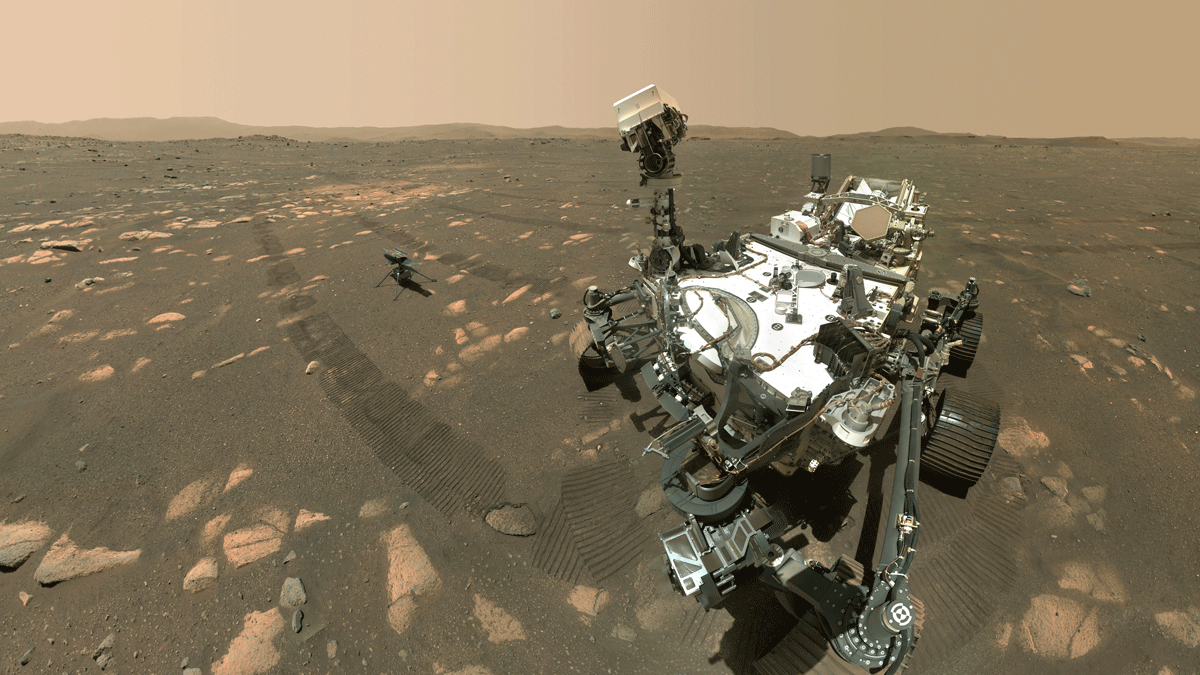
\includegraphics[width=0.5\textwidth]{imagenes/Perseverance.jpg}
    \caption{\cite{83}}
    \label{fig:perseverance}
\end{figure}

Con un peso de 1025 Kg en su lanzamiento y dimensiones similares a las de un automóvil, este dispositivo cuyo diseño está inspirado en el rover Curiosity recorre Marte en su tarea de exploración del cráter Jezero, como parte del desarrollo de una misión de la NASA. La construcción de Perseverance, el robot ilustrado en la figura \ref{fig:perseverance}, es robusta y apta para condiciones de presión y temperatura extremas \cite{2}. Asimismo, es capaz de soportar altas velocidades y aceleraciones, además del impacto de la radiación cósmica, lo hace una máquina versátil e idónea para la tarea para la que está designado.

A pesar de ello, los robots diseñados aún no poseen la capacidad de improvisación y solvencia ante problemas complejos dependientes de una gran cantidad de factores a tener en cuenta en un ambiente dinámico y hostil, como el que en esta investigación nos ocupa. En estos casos, se recurre a la presencia de  operadores para combinar la efectividad y virtudes de ambas metodologías de trabajo. De este modo, es posible omitir el riesgo implícito en el desarrollo de determinadas tareas e introducir la supervisión y control de un manipulador humano.

\subsection{Evolución del Arte}

Con el paso de los años, se ha tratado de forma continua de mejorar las metodologías utilizadas en el desarrollo de distintos procedimientos específicos para su consecución de manera óptima y en el menor período de tiempo posible, logrando así un ahorro en recursos que permite dirigir los esfuerzos disponibles en otros frentes de investigación y trabajo.

La telerrobótica, como parte de este proceso de optimización en el desempeño de ciertas actividades, es un área de la propia robótica que alude al control de máquinas a distancia haciendo uso de otras tecnologías disponibles, normalmente de carácter inalámbrico, como pueden ser Wi-Fi o Bluetooth \cite{3}. De este modo, con el uso de estas herramientas en el desarrollo de ciertas actividades, se consigue la manipulación de elementos de carácter sensible de manera segura y eficaz manteniendo al manipulador del dispositivo en un ambiente protegido.

La teleoperación, estrechamente ligada a la telerrobótica, marca sus orígenes en la industria nuclear. Encontramos un primer ejemplo de esta estrategia de trabajo en el año 1949, cuando Raymond C. Goertz, mientras trabajaba en la AEC, ideó un sistema master-slave cuyo objetivo sería manejar los productos radiactivos resultantes de la fisión nuclear. Tras este exitoso hito, el uso de los manipuladores de acoplamiento eléctrico y su potencial fueron reconocidos, sentándose así las bases de la telerrobótica moderna \cite{4}.

Más tarde, en la década de los sesenta, se trató de extrapolar los estudios realizados al campo de investigación del mar y del espacio, lo que planteó nuevos y desconocidos retos. En esta época se produjeron distintas mejoras, como el uso de cámaras y pequeños dispositivos para aumentar la telepresencia del manipulador. Pese a ello, los sistemas desarrollados denotaban deficiencias en la latencia de control, ocasionando inestabilidad \cite{5}.

Más adelante, a finales de la mencionada década, Victor Scheinman haría muestra de su brazo Stanford, un robot articulado con seis ejes. La máquina desarrollada, tenía la capacidad de seguir con precisión trayectorias señaladas en el espacio, bajo el control de una computadora \cite{6}. 

Tras los comentados inicios, y de forma continua, se producirían relevantes avances en los años sucesivos dentro de esta disciplina, rama de la robótica. Se detallan en la lista siguiente algunos de los avances más significativos, para no prolongar innecesariamente esta contextualización histórica \cite{7}:

\begin{itemize}
    \item 1971 - Formación de JIRA.
    \item 1972 - Creación del brazo del MIT.
    \item 1973 - Presentado robot  T³ con control por computadora por  Cincinnati Milacron.
    \item 1983 - Fundación de Adept Technology.
    \item 1987 - Fundación de la asociación de robótica y automatización del IEEE.
    \item 1988 - Primera Conferencia Internacional sobre Robots y Sistemas Inteligentes en Tokyo, Japón.
\end{itemize}

Observamos tras ello, como esta especialidad cobró relevancia en el panorama tecnológico global y cómo ha crecido con el paso de los años hasta nuestros días, extendiéndose en distintos ámbitos. 

\subsection{Implementaciones Actuales}
Indagando en las implementaciones actuales, se observa que el esquema básico de operación no ha sufrido una  gran cantidad de cambios. Sin embargo, las aplicaciones que implementan esta estrategia de trabajo han aumentado de manera considerable. Pese a que, se señala en gran cantidad de artículos y reseñas a la industria nuclear como principal consumidor y promotor de esta metodología de trabajo \cite{8}, podemos distinguir infinidad de aplicaciones en la actualidad, ya sean militares, industriales e incluso como complemento en distintos campos de estudio, como lo son la biología o la medicina.

\subsubsection{Aplicaciones Militares}
 A lo largo de la historia, gran cantidad de conflictos se han sucedido, siendo esta una  clara manifestación del alto nivel de sofisticación y complejidad de la gestión humana y sus avances tecnológicos. Este dominio, que permite una ingente cantidad de posibilidades, ha sido históricamente una fuente de grandes avances en distintas áreas de la ciencia, entre ellas, la telerrobótica.  

Previamente, cabe destacar que gran parte de las tecnologías de teleoperación se desarrollaron con el fin de apoyar actividades de carácter militar, y figuran entre ellas los dispositivos UAV -comúnmente conocidos como drones- y UGV -como SARGE creado por Sandia National Laboratories-, como los más conocidos. 

Entre las tareas de estos dispositivos figuran la vigilancia, la detección de enemigos, el reconocimiento del terreno, el aseguramiento de bombas, la vigilancia y el apoyo en asaltos entre otros. Tareas que, de algún modo, podrían resultar tediosas o arriesgadas para un ser humano de forma presencial \cite{9}.

\subsubsection{Aplicaciones Espaciales}
Como ya hemos comentado, algunas labores en el espacio requieren del uso de telerrobótica, como las antedichas aplicaciones; aunque las tareas que implican más riesgo para seres humanos y que a su vez nos proporcionan más información, son las de exploración. Desafortunadamente, para tareas de esta índole es prácticamente inevitable el uso de la teleoperación aún. Es por ello que las aportaciones en esta materia han sido mayúsculas por parte de este sector.

Se considera como el primer vehículo teleoperado en la superficie lunar a Lunakhod 1, en los inicios de los años 70. La tarea desempeñada por este dispositivo fue recorrer en torno a 10 kilómetros en los 11 días de duración de la misión. Como se detalló en la reseña histórica, en este tiempo los retardos en los canales de comunicación eran considerables, dificultando la misión. Sin embargo, el sistema Sojourner de la NASA, que sufrió  tiempos de retraso mucho mayores, fue teleoperado con éxito durante 7 días marcianos \cite{10}.

Las razones para el uso de la teleoperación, atisbamos, se tornan bastante claras en este contexto. Entre ellas pueden destacarse: la peligrosidad de las acciones de despegue y aterrizaje, la eliminación de los problemas de latencia, la reducción de costos -ya que los equipos de soporte vital para los astronautas son distintos de los sistemas en el espacio probados en ISS-, los problemas de radiación en superficies planetarias -puesto que son altamente perjudiciales y su mitigación puede resultar costosa- además de que las condiciones en planetas como Venus, Mercurio, Io o Titan son impracticables para nuestra anatomía, debido a las condiciones de calor y presión \cite{11}.

\subsubsection{Aplicaciones Médicas}
La telemedicina, concepto emergido en la década de los 70, surge como un método contra la lucha de las barreras geográficas, aumentando la disponibilidad de los cuidados referentes a la salud singularmente en zonas rurales y países en desarrollo. Como su nombre indica, esta disciplina de la medicina trata de prestar servicios de tratamiento o diagnóstico de enfermedades de forma remota \cite{12}. 

Podemos encontrar distintas noticias en la red acerca de los recientes avances en este campo y sus frutos. En este caso, una de las noticias que más encajan en el ámbito de esta investigación, es la prueba de que ya es posible realizar cirugías u operaciones a distancia, aunque no es la primera vez que esto se practica. 

En este caso, el cirujano Kais Assadullah Rona, demostraba cómo se puede realizar cirugía a 8,000 km de distancia haciendo uso de la red 5G, que presume de tener latencias prácticamente imperceptibles. En las imágenes, podemos ver como el operador corta la piel de una banana, para acto seguido extirpar una pequeña parte y finalmente coser el área con absoluta precisión. Con este hecho, queda patente que tareas de esta índole pueden completarse con éxito sin mayor complicación \cite{13}.
   
\subsubsection{Aplicaciones Submarinas}
Las tareas a llevar a cabo en entornos submarinos, a determinada profundidad, pueden conllevar unos altos niveles  de riesgo para el operario y un alto coste asociado. Como detallamos, el uso de autómatas en este campo también hace acto de presencia, en el mantenimiento de plataformas petrolíferas o en la industria del gas, por ejemplo. 

Para las tareas descritas, y un compendio de las mismas aún más extendido, es usual el uso de ROVs o vehículos submarinos operados a distancia. Este tipo de dispositivos son altamente maniobrables y usualmente son controlados por un equipo que opera a bordo de alguna embarcación en las proximidades o en tierra en las mismas condiciones, ya que la comunicación es cableada. Para el manejo de los brazos manipuladores se usan bombas hidráulicas, que alimentan los sistemas de torsión además \cite{14}.

En adición a lo especificado, se añaden sensores, cámaras y luces para que la experiencia del usuario manipulador sea satisfactoria, teniendo toda la información necesaria.

\subsection{Componentes del Sistema Teleoperado}

La división entre los distintos elementos que componen un sistema teleoperado no es unánimemente aceptada, ya que en algunos casos se suprimen algunas de las partes en favor de su unión con otras. En nuestro caso, tomando como referencia los artículos consultados, consideramos los principales componentes de este sistema como los descritos a continuación \cite{15}. 

\subsubsection{Operador}

Definimos como operador o manipulador a la persona que se encarga del control de las operaciones realizadas a distancia. El control que este ejerce sobre el dispositivo a teleoperar puede ser total y continuo -teniendo así la completa responsabilidad de las acciones del robot en todo momento- o alterno -ejerciendo meramente tareas de monitoreo, planificación o marcado de nuevos objetivos-.


\subsubsection{Dispositivo Controlado} 

Consideramos esta parte como la extensión del operario que trabaja en el lado de control del artefacto teleoperado. El dispositivo controlado, podrá resultar ser un robot, vehículo o sistema que trabajará en la zona remota y responderá a las órdenes de control comandadas por su manipulador.

\subsubsection{Interfaz}

Las interfaces para la teleoperación, y en general en el campo de la informática, poseen un papel de gran relevancia debido a ser las mediadoras entre el hombre y la máquina. Con este término, hacemos referencia tanto a los instrumentos que hacen posible que se efectúe el control del operador, como a cualquiera de los dispositivos que contribuyen en la retroalimentación de este. Encontramos en este punto, una clasificación en distintas categorías: las interfaces directas, multimodales o multisensoriales y de control supervisado.

\subsubsection{Control y Canales para la Comunicación}

Determinamos este componente esencial como el conjunto de medios a través de los cuales se produce el tráfico de información que será enviada y recibida a/desde el dispositivo a controlar. Este módulo será el encargado de la codificación/decodificación de los datos provenientes tanto de los dispositivos para el control como del dispositivo controlado.

\subsubsection{Sensores}

Se denominan como sensores, aquellos dispositivos que se encargan de la recolección de información tanto de la zona remota de trabajo como de la zona local de control para su posterior uso tanto en lo que a interfaces respecta como a lo que al control se refiere.

\section{Técnicas de Inmersión}

Uno de los principales modos de realimentación del entorno del ser humano es la visión. Esta capacidad que poseemos, nos permite distinguir los detalles de nuestro entorno a través de la interpretación, por parte de la corteza visual, de los rayos de luz que inciden en nuestra retina. Podríamos describir pues, la misma, como una de las principales capacidades sensoriales de los homínidos y muchos otros seres vivos.

A ese respecto, aparecen soluciones innovadoras que, ayudadas de la computación, estimulan los susodichos receptores para la consecución de una experiencia visual de contenido simulado tridimensional en tiempo real. Con ello, surgen distintos métodos dentro de este avance tecnológico con objetivos distintos y que se especifican a continuación :
\begin{itemize}
    \item Realidad virtual (VR): esta metodología de emulación del mundo percibido puede describirse como un entorno en el que se recrean escenarios y elementos con apariencia real, generados por tecnologías de carácter informático. Se hace uso, en este caso, de hardware  específico que permite al usuario la visualización de los componentes descritos en un campo de visión similar o superior al de la vista humana en tres dimensiones. Adicionalmente, la simulación obtenida puede ir acompañada de dispositivos que permitan interactuar con el medio representado, intensificando la experiencia \cite{16}.
    
    \item Realidad aumentada (AR): podemos describir esta tecnología como el compendio de métodos utilizados para la representación de un mundo enriquecido con elementos añadidos al mundo real, haciendo que este contenga información suplementaria de carácter gráfico, háptico o sonoro entre otros. Para el logro de esta experiencia se hace uso de dispositivos de distinta índole, desde smartphones a smart glasses, con la capacidad de mostrar los elementos tangibles al alcance del usuario a la vez que reconocerlos y agregarles elementos virtuales \cite{17}.  
    
    \item Realidad Mixta (MR): se alude con este término al acoplamiento entre  la realidad y la simulación mediante dispositivos electrónicos. Con esta definición, podemos inferir que los términos que describen AR y MR se tornan ambiguos entre sí y es común en la literatura su uso indistintamente.

    El propósito de la realidad mixta se fundamenta en el logro de la combinación entre VR  y AR, extendiendo el mundo tangible a la simulación virtual. Para ello, esta nueva concepción del entorno se cimenta en la creación de un modelo tridimensional de aquello que el usuario percibe como real para su posterior potenciación con contenido adicional relevante \cite{18}.
\end{itemize}

En esta sección comentaremos las distintas técnicas de inmersión disponibles, además de su desarrollo a través de los años hasta la actualidad. De forma preliminar,  estableceremos de forma directa la relación que este concepto guarda con el proyecto realizado no sin antes introducir algunos de los conceptos clave. 

Vinculando así, la presente sección con la que le precede, advertimos en varias ocasiones de que en el control de dispositivos de manera no presencial el operario necesita conocer el estado del entorno en el que el dispositivo controlado se encuentra en todo momento, para poder reaccionar ipso facto a distintas situaciones adversas que pudieran tener lugar. Esta noción, entonces, desemboca en un concepto más específico para nuestro propósito, la telepresencia.

El término telepresencia hace alusión al conjunto de técnicas que permiten que una persona perciba, gracias a los sentidos, la impresión de estar presente en el lugar deseado, creando un marco de trabajo realista para el usuario. Así pues, para lograr con la inmersión una completa experiencia de telepresencia, se hace uso de la interacción en tiempo real, una alta capacidad para la visualización del espacio simulado, acompañado de estímulos auditivos que permiten el posicionamiento y capacidades de realimentación táctil para poder sentir el hecho de colisionar, agarrar o manipular objetos en nuestro caso \cite{19}.

\subsection{Evolución del Arte}

El origen de la realidad virtual no es aceptado de forma unánime, ya que la concreción de su definición no resulta sencilla. Pese a ello, las primeras referencias a la definición moderna de este concepto se deben a la ciencia ficción.
 
Se atribuyen a Morton Leonard Heilig, pionero en este campo, los inicios de esta tecnología como la conocemos hoy día gracias a la creación de Sensorama, en 1962. Este artefacto, precursor de las tecnologías de realidad inmersiva multisensorial, más conocida en la actualidad como multimodal, es considerada una de las primeras implementaciones de la realidad virtual.

El dispositivo desarrollado incluía una pantalla estereoscópica, ventiladores, artefactos capaces de emitir distintos olores, un sistema estéreo de sonido y una silla móvil. Con ello, esta máquina tenía capacidad de simular, según se preparó como ejemplo, un viaje en motocicleta por la ciudad de Nueva York, recreando las distintas sensaciones que implicaría este, estimulando los cinco sentidos \cite{20}.

Más adelante, Ivan Sutherland, con ayuda de sus alumnos, crearía la denominada Espada de Damocles, en 1968. Este sistema, predecesor de las gafas y cascos de realidad virtual de los que hoy se hace uso, trató de utilizarse  en tareas de simulación inmersiva. El sistema desarrollado contaba con un casco -que pendía del techo debido a su peso-, un auricular, un sensor de posición de la cabeza, y distintas unidades de cálculo específicas además de un computador de uso general \cite{21}. 

En los años posteriores, este campo de estudio proporcionó instrumentos con fines médicos, militares y en la industria de la automoción. Tanto es así, que en 1979 Eric Howlett con su diseño de LEEP, se considera que sentaría las bases de los actuales cascos de realidad virtual de hoy en día. Los resultados logrados por este sistema fueron sensacionales, ya que se conseguía una realista sensación de profundidad en el amplio campo de visión en el que la imagen estereoscópica creada se extendía \cite{22}.

Más adelante, el término que designa a la Realidad virtual se popularizó a finales de la década de los ochenta por Jaron Lanier, uno de los precursores en este campo del saber. Este desarrolló algunos dispositivos de realidad virtual, entre ellos Power Glove, uno de los primeros artefactos  con esta tecnología con un precio asequible \cite{23}.

Tras este momento, gracias a los avances logrados en esta tecnología, se hizo notar un aumento en la producción de dispositivos de este tipo para el público, implicando relevantes avances en los años sucesivos dentro de este campo. Comentaremos a continuación algunos de los avances más significativos, para no prolongar innecesariamente esta contextualización histórica, como anteriormente \cite{24}:

\begin{itemize}
    \item 1988 - Cyberspace Proyect, primera implementación de VR en una computadora de bajo costo.
    \item 1990 - Sensei8 Corporation, primeros gráficos en tiempo real con mapeo de texturas.
    \item 1992 - Nicole Stenger, Angels: Primera película inmersiva e interactiva en tiempo real.
\end{itemize}


\subsection{Implementaciones Actuales}
Tratando de revisar las implementaciones actuales y los campos de aplicación para este tipo de tecnología, hallamos que en el mercado actual encuentran un buen lugar en la industria del entretenimiento y los videojuegos. No obstante, es evidente su potencial y diversos campos del saber aprovechan sus ventajas.

\subsubsection{Aplicaciones Militares}
Como indicamos anteriormente, el ámbito militar ha sido y es pionero en el uso de las tecnologías más avanzadas. En este campo de aplicación, la realidad virtual es conocida por sus aplicaciones en simuladores de entrenamiento de soldados o en simuladores de vuelo,  para pilotos inexpertos.

Se definen los simuladores de vuelo, como sistemas que tratan de replicar las condiciones de un ambiente real de trabajo en aeronaves, de la forma más precisa y realista posible. Estos sistemas de entrenamiento se crean utilizando la cabina de un avión, que más tarde será montada en una plataforma hexápoda, lo que permite un movimiento con seis grados de libertad. Estos sistemas tienen en todos los casos un coste elevado, por lo que son inaccesibles al público en general.De este modo, podrían reproducirse situaciones de fallo sin el riesgo que implica, ahorro en gastos de combustible y aeronaves, etc \cite{25}.

Por otro lado, encontramos los simuladores de tiro o simuladores de un completo campo de batalla. Haciendo uso de los mismos, los soldados pueden entrenar sus capacidades de tiro, adaptación al entorno, agrupamiento táctico y consciencia de la zona de guerra. Las ventajas de este sistema son evidentes, ya que pueden no sufrir heridas, probar distintas metodologías y entrenar de forma sucesiva sin el elevado coste asociado que ello implica. Ejemplo de ello podría ser VCTS \cite{26}.

\subsubsection{Aplicaciones Espaciales}
En el propio estudio de la Tierra, encontramos escenarios cuyas condiciones evocan las circunstancias extremas que se dan en destinos de otros mundos. Esta analogía, hace que investigadores de todo el mundo traten de comprender y aplicar las citadas tecnologías de realidad mixta y realidad virtual para la exploración del espacio exterior.

La misión BASALT, con tres distintos despliegues, se centró en tratar de realizar ciencia relevante a los campos de la biología, química y geología en entornos inhóspitos terrestres, emulando los que se darán en Marte en futuras expediciones. Con herramientas de realidad virtual y aumentada, es factible el envío de datos más completos por parte de los exploradores o los dispositivos en el terreno de aplicación para su posterior análisis por equipos de investigación. De este modo, además, los científicos en el centro de soporte podrían explorar y dirigir la misión llevada a cabo en el entorno remoto \cite{27}.

\subsubsection{Aplicaciones Médicas}
Figuran entre los casos de uso de las tecnologías citadas diversos ejemplos para la mejora en distintos procedimientos dentro de la medicina, como los listados a continuación.  

El uso de estas metódicas de trabajo, contribuyen en el campo de la educación y formación médica, especialmente en cirugía. Gracias a ello, el alumno puede realizar distintos procedimientos sobre pacientes virtuales o aprovechando las ventajas de la realidad aumentada, haciendo así la práctica más realista y productiva. 

En adición, existen estudios que ponen de manifiesto que la RV podría ser una herramienta útil para mejorar las habilidades quirúrgicas y reducir los errores de los procedimientos quirúrgicos \cite{28}.

Además de ello, ha sido testado la lidia con el agudo utilizado la realidad virtual como técnica de distracción \cite{29,30}, por consiguiente, hay estudios que proponen un papel de la RV en el manejo del dolor crónico al inducir cambios neurofisiológicos más allá de la simple distracción \cite{29,31,32}.

\subsection{Feedback Háptico}
Cuando reparamos el sentido del tacto, nos referimos a aquel que permite a los distintos tipos de organismos vivos lograr la percepción completa de los objetos que le rodean. En ausencia de éste, sería imposible la detección de propiedades como la temperatura, la textura o la dureza de las entidades de nuestro entorno. Es gracias a los receptores nerviosos que nos envuelven y el complejo sistema que comunica estos estímulos al cerebro, que somos capaces de interpretar este tipo de información de nuestro entorno para reaccionar en consecuencia.

En primer lugar, tras esta breve introducción, y para tener una completa compresión de la orientación del  proyecto; es una tarea obligada definir qué es el feedback háptico del que haremos uso. Podemos determinar la retroalimentación háptica, como la simulación por parte de un dispositivo electrónico de la sensación que nos produce el hecho de tocar o interactuar con un objeto o entidad. Dicho esto, se entiende este concepto como la forma en que un dispositivo se interrelaciona con el ser humano a través del tacto; como ya lo hacen de forma habitual por medio de la vista o el oído \cite{33}.

Esta tecnología es conocida desde largo tiempo, y ya es muy usada entre los dispositivos que usamos en el día a día, como nuestros smartphones, consolas e incluso vehículos; asistiendo en tareas como la conducción o concediéndonos una experiencia más inmersiva.

Encontramos en la actualidad diferentes usos e implementaciones con esta metódica, como lo son las plataformas en movimiento, los guantes o los dispositivos desarrollados por openHaptics de los que haremos uso \cite{34}.

\begin{itemize}
    \item Plataformas en movimiento: este tipo de ingenios de la inmersión tiene su origen en los mencionados sistemas de simulación de vuelo. En ellas, el usuario puede sentir la posición en la que se encuentra el elemento simulado, obteniendo consciencia así de cuál sería el comportamiento del dispositivo controlado en la realidad y sus limitaciones . 
    
    \item Guantes: el uso de estos dispositivos para la intensificación de la experiencia virtual es común en ambientes dinámicos que implican la interacción con objetos. Gracias a los dispositivos neumáticos que estos incorporan, el usuario es capaz de sentir la presencia y características del cuerpo en cuestión. 
\end{itemize}

El uso que se dará a esta tecnología en el seno de nuestro proyecto, tendrá el objetivo de aumentar la precisión en el control del robot que realizará las tareas de mantenimiento de forma remota. Estimamos que este, resulta un componente fundamental para una experiencia satisfactoria en el control remoto de cualquier dispositivo, al igual que la retroalimentación visual o sonora.

\section{Entorno en la Fusión Nuclear}
 
Como detallamos en la sección introductoria, la necesidad de energía es uno de los principales problemas que se tratan de solventar desde tiempos inmemoriales. Motivados por su creciente demanda, y por el cambio en las condiciones climáticas terrestres, se trata a través de la investigación y el estudio, de alcanzar formas limpias y altamente eficientes de sustituir las actuales metodologías de obtención de la misma.

En la búsqueda de procedimientos con estas características nos topamos, entre otros, con la fusión nuclear. Este proceso físico tiene lugar en el interior de las estrellas, como nuestro Sol, liberando una ingente cantidad de energía en el proceso. Tanto es así, que percibimos los efectos de la misma en forma de luz y calor, aún a ~151.47 millones de kilómetros \cite{35}. 


\begin{figure}[hbt]
    \centering
    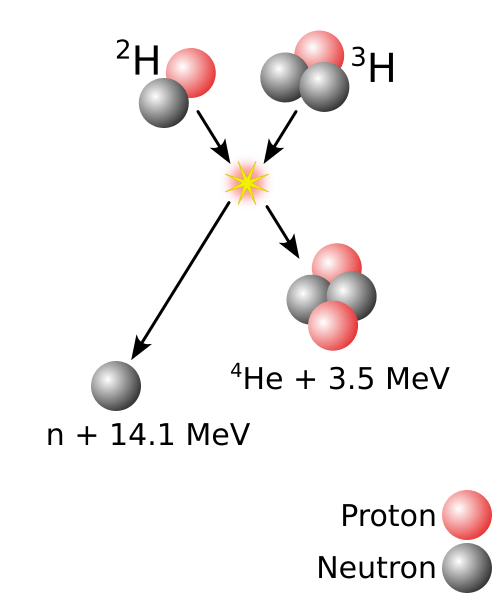
\includegraphics[width=0.3\textwidth]{imagenes/Deuterium-tritium_fusion.png}
    \caption{\cite{84}}
    \label{fig:fusion_reaction}
\end{figure}


Podemos definir la fusión nuclear pues, como el proceso físico por el que varios núcleos atómicos ligeros se unen para conformar un nuevo núcleo más pesado y nucleones, en algunos casos. Sincrónicamente, esta reacción liberará una ingente cantidad de energía -dependiendo de si la masa de los núcleos implicados supera o no la del hierro/níquel-, que permitirá al condensado resultante alcanzar el estado de plasma \cite{36}, figura \ref{fig:fusion_reaction}.

La pérdida de masa que se observa entre los reactivos y los productos, se manifestará finalmente como la energía liberada por la reacción y es explicada a través de la energía de enlace nuclear y el defecto de masa. El primer concepto, hace alusión a la cantidad de energía mínima necesaria para la descomposición de un átomo en sus protones y neutrones, mientras que el segundo, compara la diferencia entre la masa real de un átomo y la masa de sus componentes por separado, que es mayor \cite{37,38}. 

Sintetizando en gran medida, y eludiendo gran cantidad de detalles, es este último concepto es el que explica la citada energía liberada en la fusión, ya que es esta aparente pérdida de masa nuclear la responsable de la misma, como sabemos por la ecuación formulada por Albert Einstein \cite{39}: $$\Delta E=\Delta m * c^2$$.

Son varios los requisitos para conseguir las condiciones que inician y sostienen esta reacción. En primer lugar, es preciso superar la barrera de Coulomb, impulso de repulsión inducido por la fuerza electrostática -que hace que dos protones, por tener misma carga, se repelan- \cite{40}. Para lograr esto, se deben acercar los núcleos atómicos lo suficiente, de modo en que la fuerza nuclear fuerte tenga efecto, ya que en distancias del orden de 1 femtómetro su intensidad es mucho mayor, aunque decae rápidamente hasta ser imperceptible a 2.5 fm \cite{41}. 

Con el objeto de lograr esta reacción en la Tierra, es preciso replicar las condiciones que se dan en estrellas como nuestro Sol, que siguen la reacción en cadena protón-protón \cite{42}. Para ello existen varios métodos y líneas de investigación, pero en nuestro caso especificaremos las características de los reactores de clase “tokamak” de confinamiento magnético \cite{43,44}.

\begin{itemize}
    \item En primer lugar, es necesario el aporte de una ingente cantidad de energía para lograr inducir un primer estado de plasma, -implícito en la constitución de los astros, ya que poseen temperaturas cercanas a los 15 MK- y que puede conseguirse por medio de aceleradores de partículas o láseres.
    
    \item Es de capital importancia lograr un plasma suficientemente denso, para el acercamiento a través de la colisión de los citados núcleos, haciendo que la fuerza nuclear fuerte entre en juego, iniciando el proceso de fusión. (Tercer apartado)
    
    \item Para generar las condiciones de confinamiento -gracias a la gravedad y la compresión en la naturaleza-, se hace uso de campos magnéticos en volúmenes toroidales, para favorecer la estabilidad de los mismos.
\end{itemize}

La fusión es posible con todos los elementos definidos como ligeros -más livianos que el hierro/níquel-, pero la cantidad de este combustible disponible junto al hecho de que la energía a aportar en la fusión Deuterio - Tritio es considerablemente menor -debido a que la citada barrera de coulomb es mucho menor en isótopos de hidrógeno, por contener solo una carga positiva-, hacen de esta la más prometedora, aunque no se abandonan otras combinaciones posibles \cite{45}. 

Este último apartado de nuestro artículo, describe el introducido marco del trabajo realizado, exponiendo los detalles más relevantes para la consecución del objetivo que hemos planteado, además de la problemática y soluciones propuestas, en lo que a la temática de esta obra concierne.


\subsection{Proyectos Asociados}
Para comprender el marco en el que esta investigación tiene lugar, es preciso concretar el propósito de los proyectos asociados a este, cuya conjunción tiene como objetivo final la mencionada fusión nuclear.

\subsubsection{ IFMIF-DONES}
Algunas de las características de los reactores de fusión DEMO aún están por determinar, por razones que se concretan en el apartado dedicado a este proyecto. No obstante, las distintas implementaciones de reactores de este tipo, o posteriormente de fusión comercial, tendrán características comunes; como la presencia de una corriente continua de neutrones desprendidos por la fusión con una intensidad en torno a 14 Mev en el área del primer muro.

En consecuencia, la tarea de caracterización de los distintos materiales que serán utilizados en la construcción de estos dispositivos y la comprensión de cómo se modifica su estructura atómica con el paso del tiempo tras largos periodos de exposición a las antedichas circunstancias se vuelve una labor obligada.

Sin embargo, las condiciones descritas sólo pueden producirse en entornos específicos, ya que las fuentes de radiación disponibles -como lo son la fisión,  la espalación o los haces de iones- no cubren totalmente las necesidades deseadas. Es por ello, que este proyecto tratará de producir un espectro de irradiación de neutrones similar al contemplado en un proceso real de fusión -a través de una fuente basada en la fusión de deuterio y litio acelerada- con suficiente intensidad para el testeo de los materiales de los que se hará uso en las distintas instalaciones DEMO.

Con esta motivación nace IFMIF, la Instalación Internacional de Irradiación de  Materiales de  Fusión, por sus siglas en inglés. El complejo desarrollado, tratará de satisfacer los requerimientos anteriormente descritos con el uso de dos aceleradores lineales de neutrones con 40 MeV de potencia, proporcionando cada uno un haz de 125 mA. Estas fuentes de neutrones acelerados golpearán un chorro de litio líquido produciendo así un intenso flujo de neutrones de cerca de $10^{18}$ N/m²*s (unidad de viscosidad).

Anexo a este proyecto se encuentra DONES, Demo Oriented NEutron Source, cuyo objetivo es el de proveer una fuente de neutrones con suficiente intensidad y volumen de irradiación, como se ha descrito. Además de ello, se tratará de lograr las condiciones de temperatura en las zonas de flujo -250 ºC a 550 ºC-, junto a la acumulación de neutrones que tendrá lugar para producir cedencias de 20-30 (NRT-dpa) en un periodo menor a 2.5 años para 0.3L de volumen y de 50 (NRT-dpa) en lapsos de tiempo inferiores a 3 años, en volúmenes de 0.1L \cite{46}.


\subsubsection{ITER}

ITER,  Reactor Termonuclear Experimental Internacional, es un proyecto en el que colaboran más de 35 países para lograr el mayor experimento de fusión llevado a cabo, aspirando a ser el primer dispositivo de fusión en producir energía neta, es decir, generar más energía de la invertida en el calentamiento del plasma \cite{47}.

De este modo, los objetivos de este dispositivo son claros:

\begin{itemize}
    \item Producir en torno a 500 MW de energía a partir de los 50 MW de potencia inicial necesarios para el inicio de la reacción, aunque no será usado para generar energía en este caso.
    
    \item Poner a prueba los dispositivos, aún en fase experimental, que serán empleados en los futuros reactores, en condiciones semejantes a las que se darán en estos.
    
    \item Conseguir mantener un plasma con reacción deuterio-tritio, capaz de autosostenerse gracias al calor interno generado por la propia reacción, de forma estable y durante un tiempo razonablemente prolongado.
    
    \item Intentar la producción de tritio, a través del denominado “manto fértil”, que se encargará de absorber  gran parte de la energía de los neutrones resultantes de la reacción de fusión, evitando que estos alcancen las bobinas superconductoras y produciendo nuevos neutrones de menor energía que en colisión con moléculas de litio producirán tritio.
    
    \item Evidenciar las condiciones de seguridad de los dispositivos de fusión y sus bajas consecuencias medioambientales.
\end{itemize}

\subsubsection{DEMO} 

Este proyecto, como su propio nombre indica, es el último paso anterior a la fusión comercial. Este tipo de reactor, basado en ITER, deberá ser totalmente operativo a tiempo completo y  tendrá la obligación de demostrar que todas las tecnologías en las que se apoya funcionan con la fiabilidad esperada.

Las especificaciones técnicas relativas a este planteamiento no son tan claras y concisas como en el resto de la hoja de ruta descrita, ya que no hay un consenso de colaboración como en el desarrollo de ITER. No obstante, el diseño presentado por la Unión Europea es conocido y bastante documentado.

Este prototipo está llamado a generar 2 GW de energía continua con el solo uso de 80 MW de entrada térmica inyectada para el inicio de la reacción.  Para conseguir este objetivo, este artefacto deberá tener unas dimensiones un 15\% mayores a ITER y una densidad plasmática un 30\% superior.

Por supuesto, al contrario que ITER, este desarrollo sí contará con la funcionalidad de transformación de la energía liberada -aprovechando el carácter exotérmico de la reacción-, transformando el calor generado en energía eléctrica, para su posterior aporte a la red \cite{49}.
